\documentclass[10pt,pdf,hyperref={unicode}]{beamer}

\mode<presentation>
{
\usetheme{boxes}
\beamertemplatenavigationsymbolsempty

\setbeamertemplate{footline}[page number]
% \usecolortheme{seagull}
\setbeamersize{text margin left=0.5em, text margin right=0.5em}
}

\usepackage[utf8]{inputenc}
\usepackage[english, russian]{babel}
\usepackage{bm}
\usepackage{multirow}
\usepackage{ragged2e}
\usepackage{indentfirst}
\usepackage{multicol}
\usepackage{subfig}
\usepackage{amsmath,amssymb}
\usepackage{enumerate}
\usepackage{mathtools}
\usepackage{comment}

\usepackage{tikz}
\usetikzlibrary{positioning,arrows}

\tikzstyle{name} = [parameters]
\definecolor{name}{rgb}{0.5,0.5,0.5}

\newtheorem{rustheorem}{Теорема}
\newtheorem{rusdefinition}{Определение}

\AtBeginEnvironment{figure}{\setcounter{subfigure}{0}}% Resets subfigure counter at start of figure environment

\captionsetup[subfloat]{labelformat=empty}

%----------------------------------------------------------------------------------------------------------

\title[Априорное распределение параметров в задачах выбора моделей глубокого обучения]{Априорное распределение параметров \\в задачах выбора моделей глубокого обучения}
\author{А.\,В.\,Грабовой}

\institute[]{Диссертация на соискание ученой степени\\
кандидата физико-математических наук\\05.13.17~--- Теоретические основы информатики\\Научный руководитель: д.ф.-м.н. В.\,В. Стрижов\\}     
%\institute[МФТИ]{Московский Физико-Технический Институт (Государственный Университет)}
\date[2021]{\small Московский физико-технический институт\\21\;сентября\;2021\,г.}

%----------------------------------------------------------------------------------------------------------

\begin{document}
%----------------------------------------------------------------------------------------------------------
\begin{frame}
\titlepage
\end{frame}

%---------------------------------------------------------------------------------------------------------
\begin{frame}{Априорное распределение параметров моделей}
\justifying {\small
Для выбора моделей используется связный байесовский вывод. Он предполагает адекватность функции правдоподобия и априорного распределения параметров модели. 

\begin{block}{Цель исследования~---}
\justifying 
предложить метод задания априорного распределения параметров модели глубокого обучения с учетом накопленной информации о решаемой задаче.
\end{block}
\begin{block}{Исследуется проблема}
\justifying
снижения размерности пространства параметров при выборе модели. Большое число параметров и гиперпараметров влечет многоэкстремальность и невыпуклость задачи оптимизации, а также её высокую вычислительную сложность.
\end{block}
\begin{block}{Требуется предложить}
\justifying
%\begin{enumerate}[1)]
%\item  
1)~метод выбора модели, основанный на использовании привилегированной и накопленной информации,
\\%\item  
2)~метод сопоставления структур параметрических моделей,% на основе байесовского вывода,
\\%\item  
3)~метод снижения размерности пространства параметров моделей глубокого обучения.
%\end{enumerate}
\end{block}
\begin{block}{Используются методы}
\justifying
связного байесовского вывода. Для назначения априорного распределения параметров при выборе моделей глубокого обучения используется априорная экспертная информация и распределение параметров ранее полученных моделей.
\end{block}
}
\end{frame}
%\end{document}
%---------------------------------------------------------------------------------------------------------

\begin{frame}{Оптимизация ученика на основе учителя\footnotemark~и привилегированных признаков\footnotemark}
\justifying
Заданы:
\begin{enumerate}
    \item[1)] признаки~$\mathbf{x}_i \in \mathbb{R}^{n}$ и привилегированные признаки~$\mathbf{x}^*_i \in \mathbb{R}^{n^*}$,
    \item[2)] целевая переменная~$y_i \in \mathbb{Y}$,
    \item[3)] индексы объектов, для которых известна привилегированная информация $\mathcal{I},$ а для которых она не известна $\bar{\mathcal{I}}$.
\end{enumerate}

Функции учителя~$\mathbf{f}:\mathbb{R}^{n^*} \to \mathbb{Y}^\prime$ и ученика~$\mathbf{g}:\mathbb{R}^{n} \to \mathbb{Y}^\prime$ --- пространство оценок.

Ответы $\mathbf{s}_i = \mathbf{f}\bigr(\mathbf{x}_i^*\bigr)$ функции $\mathbf{f}$ для объектов~$\mathbf{x}^*_i$.

\bigskip

Требуется выбрать модель ученика~$\mathbf{g}$ из множества
\[
	\mathfrak{G} = \left\{\mathbf{g}| \mathbf{g}:\mathbb{R}^{n} \to \mathbb{Y}^\prime\right\}.
\]
Оптимизационная задача:
\[
	\mathbf{g} = \arg\min_{\mathbf{g} \in \mathfrak{G}} \mathcal{L}\bigr(\mathbf{g}, \mathbf{f}, \mathbf{X}, \mathbf{X}^{*}, \mathbf{y}\bigr),
\]
где $\mathcal{L}$ функция ошибки.

\bigskip

\footnotetext[1]{\textit{Hinton G., Vinyals O., Dean J.} Distilling the Knowledge in a Neural Network // NIPS, 2015.}
\footnotetext[2]{\textit{Lopez-Paz D., Bottou L., Scholkopf B., Vapnik V.} Unifying Distillation and Privileged Information // ICLR, 2016.}
\end{frame}

%----------------------------------------------------------------------------------------------------------

\begin{frame}
\justifying
\frametitle<1>{Базовая постановка задачи машинного обучения}
\frametitle<2>{Априорное распределение параметров}
\frametitle<3>{Байесовская дистилляция модели}

\begin{minipage}[t][3cm][t]{\textwidth}
\only<1>{\begin{figure}[h!]
    \begin{center}
        
\includegraphics[width=1.0\textwidth]{figures/introdigram_low.png}
    \end{center}
\end{figure}}

\only<2>{\begin{figure}[h!]
    \begin{center}
        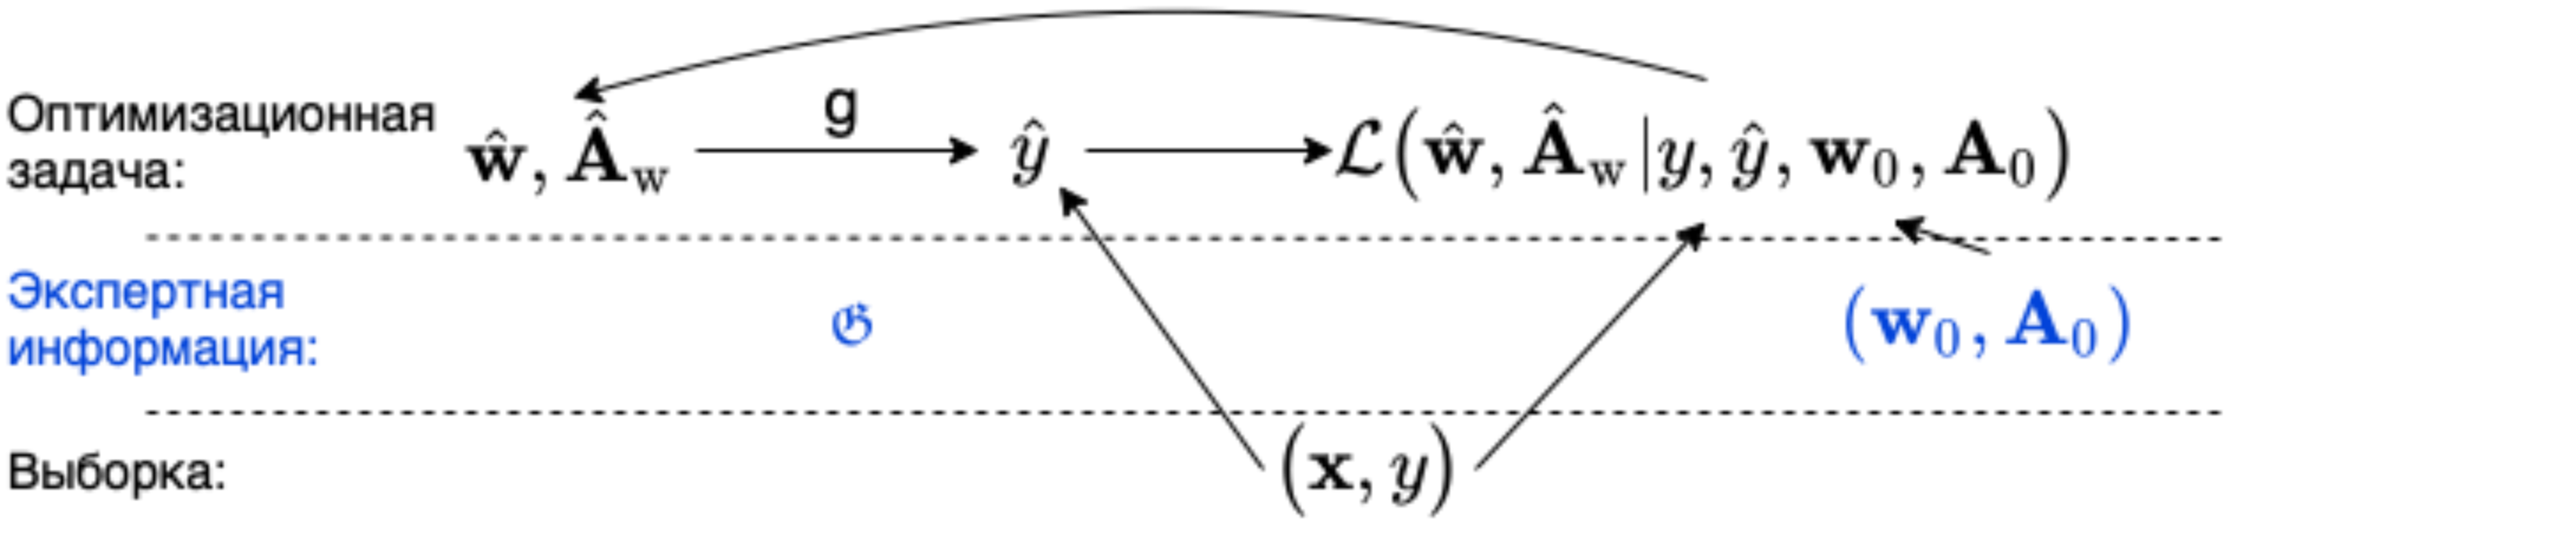
\includegraphics[width=1.0\textwidth]{figures/introdigram.png}
    \end{center}
\end{figure}}

\only<3>{\begin{figure}[h!]
    \begin{center}
        
\includegraphics[width=1.0\textwidth]{figures/introdigram_large}
    \end{center}
\end{figure}}
\end{minipage}
\vfill

\begin{itemize}
    \item \only<1-2>{Задана выборка:
$
	\mathfrak{D} = \left\{\mathbf{x}_i, y_i\right\}_{i=1}^{m}, \quad 
	\mathbf{x}_{i} \in \mathbb{R}^{n}, \quad y_i \in \mathbb{Y},
$ где~$m$~число объектов, $n$~число признаков.
}
\only<3>{Задана выборка:
$
	\mathfrak{D} = \left\{\mathbf{x}_i, {\color{blue}\mathbf{x}_i^{*}}, y_i\right\}_{i=1}^{m}, 
	\quad \mathbf{x}_{i} \in \mathbb{R}^{n}, 
	{\color{blue} \quad \mathbf{x}_{i}^{*} \in \mathbb{R}^{n^{*}}},
	\quad y_i \in \mathbb{Y},
$ где~$m$~число объектов, $n$~число признаков, {\color{blue}$n^*$}~число признаков}
    \item \only<1-2>{Модель:
$
    \mathfrak{G} = \left\{g | g : \mathbb{R}^{n}\times \mathbb{R}^{n_{w}} \to \mathbb{Y} \right\}.
$}
\only<3>{Модель:
$
    \mathfrak{G} = \left\{g | g : \mathbb{R}^{n}\times \mathbb{R}^{n_{w}} \to \mathbb{Y} \right\},
{\color{blue}
    \quad \mathfrak{F} = \left\{f | f : \mathbb{R}^{n^{*}}\times \mathbb{R}^{n_{w}^{*}} \to \mathbb{Y} \right\}.
}
$}
    \item<2-3> \only<2>{\color{blue}
Априорное распределение параметров:
$
    \mathbf{w} \sim \mathcal{N}\bigr(\mathbf{w}_0, \mathbf{A}_0\bigr).
$
}\only<3>{
Априорное распределение параметров:
$
    \mathbf{w} \sim \mathcal{N}\bigr({\color{blue}\mathbf{w}_0\bigr(\hat{\mathbf{u}}, \hat{\mathbf{A}}_{\text{u}}\bigr)}, {\color{blue}\mathbf{A}_0\bigr(\hat{\mathbf{u}}, \hat{\mathbf{A}}_{\text{u}}\bigr)}\bigr).
$}
    \item \only<1>{Прогноз:
$
    \hat{y} = g\bigr(\mathbf{x}, \hat{\mathbf{w}}).
$}
\only<2>{Прогноз:
$
    \hat{y} = g\bigr(\mathbf{x}, \hat{\mathbf{w}})
$}
\only<3>{Прогноз:
$
    \hat{y} = g\bigr(\mathbf{x}, \hat{\mathbf{w}}),
{\color{blue}
    \quad
    s = f\bigr(\mathbf{x}^{*}, \hat{\mathbf{u}}).
}
$}
    \item \only<1>{Функция потерь:
$
    \mathcal{L}\bigr(\hat{\mathbf{w}},\hat{\mathbf{A}}_{\text{w}}|y, \hat{y}\bigr).
$}
\only<2>{Функция потерь:
$
    \mathcal{L}\bigr(\hat{\mathbf{w}},\hat{\mathbf{A}}_{\text{w}}|y, \hat{y}, {\color{blue}\mathbf{w}_0, \mathbf{A}_0}\bigr).
$}
\only<3>{Функция потерь:
$
    \mathcal{L}\bigr(\hat{\mathbf{w}},\hat{\mathbf{A}}_{\text{w}}|{\color{blue} s, }y, \hat{y}, {\color{blue}\mathbf{w}_0, \mathbf{A}_0}\bigr).
$}
    \item \only<1-2>{Оптимизационная задача:
\[
    \hat{\mathbf{w}}, \hat{\mathbf{A}}_{w} = \arg \min_{\mathbf{w} \in \mathbb{R}^{n_{w}}, \mathbf{A} \in \mathbb{R}^{n_{w}\times n_{w}}} \mathcal{L}\bigr(\mathbf{w},\mathbf{A}_{\text{w}}|y, \hat{y}\bigr).
\]}
\only<3>{Оптимизационная задача:
\[
    \hat{\mathbf{w}}, \hat{\mathbf{A}}_{w} = \arg \min_{\mathbf{w} \in \mathbb{R}^{n_{w}}, \mathbf{A} \in \mathbb{R}^{n_{w}\times n_{w}}} \mathcal{L}\bigr(\hat{\mathbf{w}},\hat{\mathbf{A}}_{\text{w}}|{\color{blue} s, }y, \hat{y}, {\color{blue}\mathbf{w}_0, \mathbf{A}_0}\bigr).
\]}
\end{itemize}


\end{frame}

\begin{comment}
%----------------------------------------------------------------------------------------------------------

\begin{frame}{Базовая постановка задачи машинного обучения}
\justifying

\begin{figure}[h!]

\includegraphics[width=1.0\textwidth]{figures/introdigram_low.png}
\end{figure}

Задана выборка:
$
	\mathfrak{D} = \left\{\mathbf{x}_i, y_i\right\}_{i=1}^{m}, \quad 
	\mathbf{x}_{i} \in \mathbb{R}^{n}, \quad y_i \in \mathbb{Y},
$
где~$m$~число объектов, $n$~число признаков.\\[1mm]
Модель:
$
    \mathfrak{G} = \left\{g | g : \mathbb{R}^{n}\times \mathbb{R}^{n_{w}} \to \mathbb{Y} \right\}.
$\\[1mm]
Прогноз:
$
    \hat{y} = g\bigr(\mathbf{x}, \hat{\mathbf{w}}).
$\\[1mm]
Функция потерь:
$
    \mathcal{L}\bigr(\hat{\mathbf{w}},\hat{\mathbf{A}}_{\text{w}}|y, \hat{y}\bigr).
$\\[1mm]
Оптимизационная задача:
\[
    \hat{\mathbf{w}}, \hat{\mathbf{A}}_{w} = \arg \min_{\mathbf{w} \in \mathbb{R}^{n_{w}}, \mathbf{A} \in \mathbb{R}^{n_{w}\times n_{w}}} \mathcal{L}\bigr(\mathbf{w},\mathbf{A}_{\text{w}}|y, \hat{y}\bigr).
\]
\end{frame}

%----------------------------------------------------------------------------------------------------------


\begin{frame}{Априорное распределение параметров}
\justifying

\begin{figure}[h!]
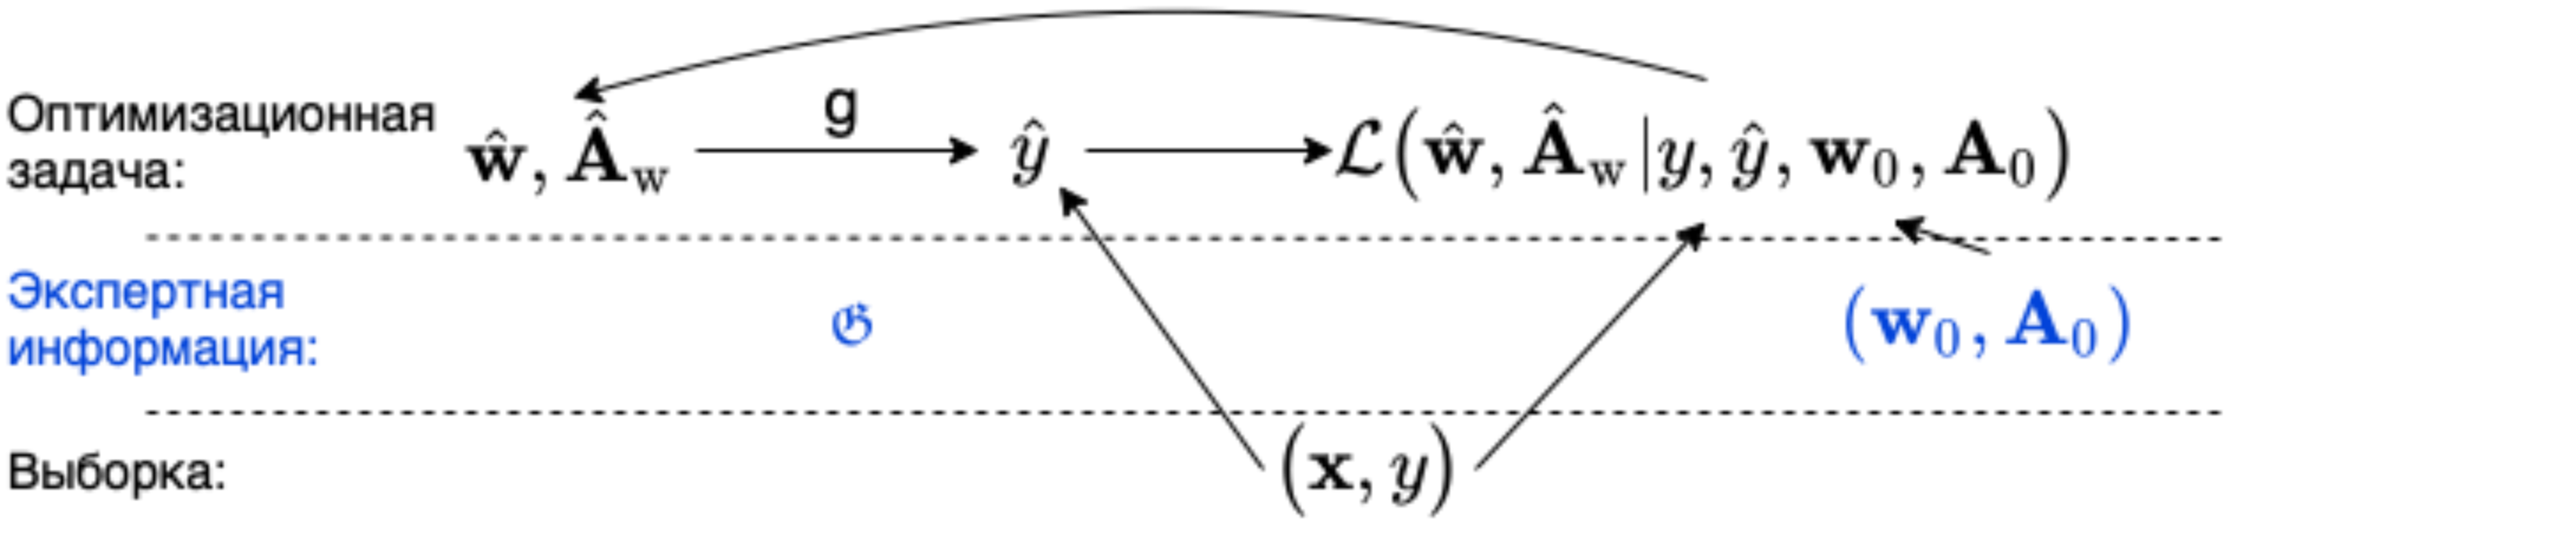
\includegraphics[width=1.0\textwidth]{figures/introdigram.png}
\end{figure}

Задана выборка:
$
	\mathfrak{D} = \left\{\mathbf{x}_i, y_i\right\}_{i=1}^{m}, \quad 
	\mathbf{x}_{i} \in \mathbb{R}^{n}, \quad y_i \in \mathbb{Y},
$
где~$m$~число объектов, $n$~число признаков.\\[1mm]
Модель:
$
    \mathfrak{G} = \left\{g | g : \mathbb{R}^{n}\times \mathbb{R}^{n_{w}} \to \mathbb{Y} \right\}.
$\\[1mm]
{\color{blue}
Априорное распределение параметров модели:
$
    \mathbf{w} \sim \mathcal{N}\bigr(\mathbf{w}_0, \mathbf{A}_0\bigr).
$\\[1mm]
}
Прогноз:
$
    \hat{y} = g\bigr(\mathbf{x}, \hat{\mathbf{w}}).
$\\[1mm]
Функция потерь:
$
    \mathcal{L}\bigr(\hat{\mathbf{w}},\hat{\mathbf{A}}_{\text{w}}|y, \hat{y}, {\color{blue}\mathbf{w}_0, \mathbf{A}_0}\bigr).
$\\[1mm]
Оптимизационная задача:
\[
    \hat{\mathbf{w}}, \hat{\mathbf{A}}_{w} = \arg \min_{\mathbf{w} \in \mathbb{R}^{n_{w}}, \mathbf{A} \in \mathbb{R}^{n_{w}\times n_{w}}} \mathcal{L}\bigr(\hat{\mathbf{w}},\hat{\mathbf{A}}_{\text{w}}|y, \hat{y}, {\color{blue}\mathbf{w}_0, \mathbf{A}_0}\bigr).
\]
\end{frame}

%----------------------------------------------------------------------------------------------------------

\begin{frame}{Байесовская дистилляция модели}
\justifying
\begin{figure}[h!]

\includegraphics[width=1.0\textwidth]{figures/introdigram_large}
\end{figure}

Задана выборка:
$
	\mathfrak{D} = \left\{\mathbf{x}_i, {\color{blue}\mathbf{x}_i^{*}}, y_i\right\}_{i=1}^{m}, 
	\quad \mathbf{x}_{i} \in \mathbb{R}^{n}, 
	{\color{blue}\quad \mathbf{x}_{i}^{*} \in \mathbb{R}^{n^{*}}},
	\quad y_i \in \mathbb{Y}.
$\\[1mm]
Модели ученика и учителя:
$
    \mathfrak{G} = \left\{g | g : \mathbb{R}^{n}\times \mathbb{R}^{n_{w}} \to \mathbb{Y} \right\},
{\color{blue}
    \quad \mathfrak{F} = \left\{f | f : \mathbb{R}^{n^{*}}\times \mathbb{R}^{n_{w}^{*}} \to \mathbb{Y} \right\}.
}
$\\[1mm]
{\color{blue}
Задана оптимальная функция учителя~$f \in \mathfrak{F}.$
}
\\[1mm]
Априорное распределение параметров модели:
$
    \mathbf{w} \sim \mathcal{N}\bigr({\color{blue}\mathbf{w}_0\bigr(\hat{\mathbf{u}}, \hat{\mathbf{A}}_{\text{u}}\bigr)}, {\color{blue}\mathbf{A}_0\bigr(\hat{\mathbf{u}}, \hat{\mathbf{A}}_{\text{u}}\bigr)}\bigr).
$\\[1mm]
Прогноз:
$
    \hat{y} = g\bigr(\mathbf{x}, \hat{\mathbf{w}}).
{\color{blue}
    \quad
    s = f\bigr(\mathbf{x}^{*}, \hat{\mathbf{u}}).
}
$\\[1mm]
Функция потерь:
$
    \mathcal{L}\bigr(\hat{\mathbf{w}},\hat{\mathbf{A}}_{\text{w}}|{\color{blue} s, }y, \hat{y}, {\color{blue}\mathbf{w}_0, \mathbf{A}_0}\bigr).
$\\[1mm]
Оптимизационная задача:
\[
    \hat{\mathbf{w}}, \hat{\mathbf{A}}_{w} = \arg \min_{\mathbf{w} \in \mathbb{R}^{n_{w}}, \mathbf{A} \in \mathbb{R}^{n_{w}\times n_{w}}} \mathcal{L}\bigr(\hat{\mathbf{w}},\hat{\mathbf{A}}_{\text{w}}|{\color{blue} s, }y, \hat{y}, {\color{blue}\mathbf{w}_0, \mathbf{A}_0}\bigr).
\]
\end{frame}
\end{comment}

%----------------------------------------------------------------------------------------------------------
\begin{frame}{Привилегированное обучение {\color{red}В.\,Н.\;Вапника} и \\ \hfill\hfill\hfill дистилляция~{\color{blue}Дж.\;Хинтона}}
\justifying
Заданы:
\begin{enumerate}
	\item[1)] {\color{blue} $\mathbf{x}^*_i = \mathbf{x}_i$}, {\color{red} $\mathbf{x}^*_i \not= \mathbf{x}_i$} для всех $i \in \{1, 2, \cdots, m\}$,
	\item[2)] $y_i \in \mathbb{Y}=\{1, \cdots, K\}, \quad \mathbb{Y}^\prime=\mathbb{R}^{K}$.
\end{enumerate}

Параметрические семейства учителя и ученика:
\[
%\setlength\abovedisplayskip{0pt}
\mathfrak{F}^{\color{red}*}_{\text{cl}} = \left\{\mathbf{f}| \mathbf{f} = \text{softmax}\bigr(\mathbf{v}^{\color{red}*}\bigr(\mathbf{x}^{\color{red}*}\bigr)/T\bigr), \quad \mathbf{v}^{\color{red}*}: \mathbb{R}^{n^{\color{red}*}} \to \mathbb{R}^K \right\},
%\setlength\belowdisplayskip{0pt}
\]
\[
%\setlength\abovedisplayskip{0pt}
\mathfrak{G}_{\text{cl}} = \left\{\mathbf{g}| \mathbf{g} = \text{softmax}\bigr(\mathbf{z}\bigr(\mathbf{x}\bigr)/T\bigr), \quad \mathbf{z}: \mathbb{R}^n \to \mathbb{R}^K \right\},
%\setlength\belowdisplayskip{0pt}
\]
где~$\mathbf{z},\mathbf{v}^{\color{red}*}$~--- это дифференцируемые по параметрам функции заданной структуры, $T$~--- параметр температуры.

Функция ошибки
\[
\setlength\abovedisplayskip{0pt}
\begin{aligned}
   \mathcal{L}_\text{st}\bigr(\mathbf{g}\bigr) = &-\sum_{i=1}^{m}\underbrace{{\sum_{k=1}^{K}y^k_i\log\mathbf{g}\bigr(\mathbf{x}_i\bigr)\bigr|_{T=1}}}_{\text{исходная функция потерь}}- \sum_{i=1}^{m}\underbrace{{\sum_{k=1}^{K}\mathbf{f}\bigr(\mathbf{x}^{\color{red}*}_i\bigr)\bigr|_{T=T_0}\log\mathbf{g}\bigr(\mathbf{x}_i\bigr)\bigr|_{T=T_0}}}_{\text{слагаемое дистилляции}},
\end{aligned}
\setlength\belowdisplayskip{0pt}
\]
где~$\cdot\bigr|_{T=t}$ фиксирует температуру~$T$.

%Оптимальная модель~$\mathbf{g}$ выбирается из класса~$\mathfrak{G}_{\text{cl}}$,
Оптимальная модель выбирается из класса,
%\[\setlength\abovedisplayskip{0pt}
$\hat{\mathbf{g}} = \arg\min_{\mathbf{g} \in \mathfrak{G}_{\text{cl}}} \mathcal{L}_\text{st}\bigr(\mathbf{g}\bigr).$
%\setlength\belowdisplayskip{0pt}\]
\end{frame}
%----------------------------------------------------------------------------------------------------------
\begin{frame}{Вероятностная постановка задачи дистилляции}
\justifying
Гипотеза порождения данных:
\begin{enumerate}
	\item[1)] задано распределение целевой переменной~$p\bigr(y_i|\mathbf{x}_i, \mathbf{g}\bigr)$,
	\item[2)] задано совместное распределение~$p\bigr(y_i, \mathbf{s}_i|\mathbf{x}_i, \mathbf{g}\bigr)$,
	\item[3)] для всех $i \in \mathcal{I}$ элементы $y_i$ и $\mathbf{s}_i$ являются зависимыми величинами,
	\item[4)] если $|\mathcal{I}|=0$ то решение равно решению максимума правдоподобия.
\end{enumerate}
Совместное правдоподобие истинных меток и меток учителя:
\[
\setlength\abovedisplayskip{0pt}
p\bigr(\mathbf{y}, \mathbf{S}|\mathbf{X}, \mathbf{g}, \mathcal{I}\bigr)=\prod_{i\not\in \mathcal{I}}p\bigr(y_i|\mathbf{x}_i, \mathbf{g}\bigr)\prod_{i\in \mathcal{I}}p\bigr(y_i, \mathbf{s}_i|\mathbf{x}_i, \mathbf{g}\bigr).
\setlength\belowdisplayskip{0pt}
\]

\begin{columns}
\column{0.55\textwidth}
Задача оптимизации:
\[
\setlength\abovedisplayskip{0pt}
\mathbf{g} = \arg\max_{\mathbf{g} \in \mathfrak{G}} p\bigr(\mathbf{y}, \mathbf{S}|\mathbf{X}, \mathbf{g}, \mathcal{I}\bigr),
\setlength\belowdisplayskip{0pt}
\]
имеет вид:
\[
\setlength\abovedisplayskip{0pt}
\begin{aligned}
\sum_{i\not\in \mathcal{I}}\log p\bigr(y_i|\mathbf{x}_i, \mathbf{g}\bigr) &+ \left(1-\lambda\right)\sum_{i\in \mathcal{I}}\log p\bigr(y_i|\mathbf{x}_i, \mathbf{g}\bigr) \\
&+ \lambda\sum_{i\in \mathcal{I}}\log p\bigr(\mathbf{s}_i|\mathbf{x}_i, \mathbf{g}\bigr),
\end{aligned}
\setlength\belowdisplayskip{0pt}
\]
где~$\lambda \in [0,1]$ --- метапараметр.
\column{0.4\textwidth}
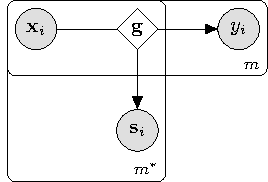
\includegraphics[width=\textwidth]{figures/proba_model}
\end{columns}

\end{frame}

%----------------------------------------------------------------------------------------------------------
\begin{frame}{Вероятностная постановка задачи классификации}
\justifying
Заданы:
\begin{enumerate}
	\item[1)] учитель $\mathbf{f}\in\mathfrak{F}_{\text{cl}}^{*}$ и ученик~$\mathbf{g}\in\mathfrak{G}_{\text{cl}}$,
	\item[2)] распределение истинных меток~$p\bigr(y|\mathbf{x}, \mathbf{g}\bigr) = \text{Cat}\bigr(\mathbf{g}\bigr(\mathbf{x}\bigr)\bigr)$,
	\item[3)] распределение ответов учителя~$p\bigr(\mathbf{s}|\mathbf{x}, \mathbf{g}\bigr) = C\prod_{k=1}^{K}g_k\bigr(\mathbf{x}\bigr)^{s^k}, \quad C < \infty,$
\end{enumerate}
\[
\setlength\abovedisplayskip{0pt}
\begin{aligned}
&\hat{\mathbf{g}} = \arg\max_{\mathbf{g}\in \mathfrak{G}} \sum_{i\not\in \mathcal{I}}\sum_{k=1}^{K}y_i^k\log g_k\bigr(\mathbf{x}_i\bigr)\bigr|_{T=1} 
+ \left(1-\lambda\right)\sum_{i\in \mathcal{I}}\sum_{k=1}^{K}y_i^k\log g_k\bigr(\mathbf{x}_i\bigr)\bigr|_{T=1} \\
&+ \lambda\sum_{i\in \mathcal{I}}\sum_{k=1}^{K}s_{i,k}\log g_k\bigr(\mathbf{x}_i\bigr)\bigr|_{T=T_0} 
+ \lambda \sum_{i\in \mathcal{I}}\sum_{k=1}^{K}\left(\log g_k\bigr(\mathbf{x}_i\bigr)\bigr|_{T=T_0} + \log\log\frac{1}{g_k\bigr(\mathbf{x}_i\bigr)}\bigr|_{T=T_0}\right).
\end{aligned}
\setlength\belowdisplayskip{0pt}
\]

\begin{rustheorem}[Грабовой, 2020]
\label{theorem:st:dist}
Пусть всех $k$ выполняется $1 > 1- \varepsilon > g_k\bigr(\mathbf{x}\bigr) > \varepsilon > 0,$ тогда при
\[
\setlength\abovedisplayskip{0pt}
C=\left(-1\right)^{K}\frac{K^{K/2}}{2^{K(K-1)/2}}\prod_{k=1}^{K}g_k\bigr(\mathbf{x}\bigr)\log g_k\bigr(\mathbf{x}\bigr)
\setlength\belowdisplayskip{0pt}
\]
функция $p\bigr(\mathbf{s}|\mathbf{x}, \mathbf{g}\bigr) = C\prod_{k=1}^{K}g_k\bigr(\mathbf{x}\bigr)^{s^k}$ является плотностью распределения.
\end{rustheorem}

\end{frame}
%----------------------------------------------------------------------------------------------------------
\begin{frame}{Вероятностная постановка задачи регрессии}
\justifying
\begin{enumerate}[1)]
	\item учитель~$f\in\mathfrak{F}_{\text{rg}}^{*}= \left\{f| f = \mathbf{v}^*\bigr(\mathbf{x}^*\bigr), \quad \mathbf{v}^*: \mathbb{R}^{n^*} \to \mathbb{R} \right\}$,
	\item ученик~$g\in\mathfrak{G}_{\text{rg}} = \left\{g| g = \mathbf{z}\bigr(\mathbf{x}\bigr), \quad \mathbf{z}: \mathbb{R}^n \to \mathbb{R} \right\}$,
	\item распределение истинных меток $p\bigr(y|\mathbf{x}, g\bigr) = \mathcal{N}\bigr(y|g\bigr(\mathbf{x}\bigr), \sigma\bigr)$,
	\item распределения меток учителя $p\bigr(s| \mathbf{x}, g\bigr) = \mathcal{N}\bigr(s|g\bigr(\mathbf{x}\bigr), \sigma_s\bigr).$
\end{enumerate}
Оптимизационная задача:
\[
\setlength\abovedisplayskip{0pt}
\begin{aligned}
\hat{g} = \arg\min_{g\in \mathfrak{G}} & \sum_{i\not\in \mathcal{I}}\sigma^2\left(y_i-g\bigr(\mathbf{x}_i\bigr)\right)^2 \\
&+ \left(1-\lambda\right)\sum_{i\in \mathcal{I}}\sigma^2\left(y_i-g\bigr(\mathbf{x}_i\bigr)\right)^2 + \lambda\sum_{i\in \mathcal{I}}\sigma_s^2\left(s_i-g\bigr(\mathbf{x}_i\bigr)\right)^2.
\end{aligned}
\setlength\belowdisplayskip{0pt}
\]

\begin{rustheorem}[Грабовой, 2020]
\label{theorem:st:reg}
Пусть~$\mathfrak{G}_{rg}$ --- класс линейных функций~$g\bigr(\mathbf{x}\bigr) = \mathbf{w}^{\mathsf{T}}\mathbf{x}.$ Тогда решение оптимизационной задачи эквивалентно решению задачи линейной регрессии $\mathbf{y''} = \mathbf{X}\mathbf{w} + \bm{\varepsilon},~\bm{\varepsilon} \sim \mathcal{N}\bigr(\mathbf{0}, \bm{\Sigma}\bigr)$ ,
где $\bm{\Sigma}^{-1}=\text{diag}\bigr(\bm{\sigma'}\bigr)$ и $\mathbf{y''}$ имеют следующий вид:
\[
\setlength\abovedisplayskip{0pt}
\begin{aligned}
\sigma'_{i} = \begin{cases}
\sigma^2,~\text{если}~i \not \in \mathcal{I}\\
\left(1-\lambda\right)\sigma^2+\lambda\sigma_s^2,~\text{иначе},
\end{cases}
\mathbf{y}'' = \bm{\Sigma}\mathbf{y}', \quad
y'_i = \begin{cases}
\sigma^2y_i,~\text{если}~i \not \in \mathcal{I}\\
\left(1-\lambda\right)\sigma^2y_i+\lambda\sigma_s^2s_i,~\text{иначе}.
\end{cases}
\end{aligned}
\setlength\belowdisplayskip{0pt}
\]
\end{rustheorem}
\end{frame}

%----------------------------------------------------------------------------------------------------------

\begin{frame}{Байесовская постановка задачи дистилляции}

Задана модель учителя, суперпозиция
\[
%\begin{aligned}
\mathbf{f}\bigr(\mathbf{x}\bigr) = \bm{\sigma} \circ \mathbf{U}_T\bm{\sigma} \circ \mathbf{U}_{T-1}\bm{\sigma} \circ \cdots \circ \mathbf{U}_1\mathbf{x},
%\end{aligned}
\]
где~$\mathbf{U}$ матрицы линейных отображений,~$\bm{\sigma}$ монотонная вектор-функция. Параметры учителя фиксированы
\[
\begin{aligned}
\mathbf{u} = \text{vec}\bigr(\left[\mathbf{U}_T, \mathbf{U}_{T-1}, \cdots \mathbf{U}_1\right]\bigr).
\end{aligned}
\]
На основе выборки~$\left\{\mathbf{x}_i, y_i\right\}_{i=1}^{m}$ и значений учителя~$\mathbf{f}(\hat{\mathbf{u}},\mathbf{x})$ требуется выбрать модель ученика:
\[
\begin{aligned}
\mathbf{g}\bigr(\mathbf{x}\bigr) = \bm{\sigma} \circ \mathbf{W}_L\bm{\sigma} \circ \cdots \circ \mathbf{W}_1\mathbf{x}, \quad \mathbf{W}_l \in \mathbb{R}^{n_s \times n_{s-1}},
\end{aligned}
\]
где~$\mathbf{W}$,~$\bm{\sigma}$ вводятся как и отображения учителя. Задача выбора модели~$\mathbf{g}$ состоит в оптимизации вектора~$\mathbf{w}$.  Решается  вариационным выводом
\[
\begin{aligned}
\hat{\mathbf{w}}, \hat{\bm{\mu}}, \hat{\bm{\Sigma}} = \arg \min_{\bm{\mu}, \bm{\Sigma}, \mathbf{w}} \text{D}_{\text{KL}}\bigr(q\bigr(\mathbf{w}|\bm{\mu}, \bm{\Sigma}\bigr)||p\bigr(\mathbf{w}|\mathbf{A}\bigr)\bigr) - \sum_{i=1}^{m}\log p\bigr(y_i|\mathbf{x}_{i}, \mathbf{w}\bigr).
\end{aligned}
\]
Априорное распределение~$p\bigr(\mathbf{w}|\mathbf{A}\bigr)$ задается как функция от апостериорного распределения параметров учителя~$p\bigr(\mathbf{u}|\mathbf{X}, \mathbf{y}\bigr)$.  Оно задано,
\[
\setlength\abovedisplayskip{0pt}
\begin{aligned}
p\bigr(\mathbf{u}|\mathbf{X}, \mathbf{y}\bigr) = \mathcal{N}\bigr(\mathbf{m}, \bm{\Sigma}\bigr).
\end{aligned}
\]
{\it \color{red}Проблема: пространства параметров учителя и ученика не совпадают.}
\end{frame}


%----------------------------------------------------------------------------------------------------------
\begin{frame}{Сопоставление структурных параметров}
%\begin{rusdefinition}
Множество структурных параметров задает вид суперпозиции моделей~$\mathbf{f}, \mathbf{g}$.
%\end{rusdefinition}

\begin{rusdefinition}
Сопоставление параметрических моделей~--- изменение структуры одной или нескольких моделей в результате которого векторы параметров моделей различных структур лежат в одном пространстве.
\end{rusdefinition}


\textbf{Пространства параметров совпадают}
\begin{itemize}
    \item[---] число слоев совпадает $L=T$,
    \item[---] размеры соответствующих слоев совпадают,
\end{itemize}
тогда
\[
p\bigr(\mathbf{w}|\mathbf{A}\bigr) = p\bigr(\mathbf{w}|\mathbf{X}, \mathbf{y}\bigr).
\]

\textbf{Пространства параметров не совпадают}
\begin{itemize}
    \item[---] выполняется сопоставление моделей учителя~$\mathbf{g}$ и ученика~$\mathbf{f}$,
    \item[---] апостериорное распределение учителя~$p\bigr(\mathbf{u}|\mathbf{X}, \mathbf{y}\bigr)$ назначается априорным распределением ученика~$p\bigr(\mathbf{w}|\mathbf{A}\bigr)$.
\end{itemize}

\end{frame}

%----------------------------------------------------------------------------------------------------------
\begin{frame}{Размеры скрытых слоев учителя и ученика отличаются}

Преобразования $t$-го слоя учителя:
\[
\begin{aligned}
\phi\bigr(t, \mathbf{u}\bigr) : \mathbb{R}^{\text{p}_{\text{tr}}} \to \mathbb{R}^{\text{p}_{\text{tr}}-2n_t}
\end{aligned}
\]
описывает удаление одного нейрона из~$t$-го слоя. Новый вектор параметров $\bm{\upsilon} =  \phi\bigr(t, \mathbf{u}\bigr),$ а элементы вектора, которые были удалены как $\bar{\bm{\upsilon}}$

\begin{rustheorem}[Грабовой, 2021]
Пусть выполняются следующие условия:
\begin{enumerate}[1)]
\item апостериорное распределение параметров $p\bigr(\mathbf{u}|\mathfrak{D}\bigr) = \mathcal{N}\bigr(\mathbf{m}, \bm{\Sigma}\bigr),$
\item число слоев модели учителя равняется числу слоев модели ученика $T=L$,
\item размеры соответствующих слоев не совпадают, другими словами, для всех $t, l,$ таких что $t=l,$ выполняется $n_t \leq n_l.$
\end{enumerate}
Тогда апостериорное распределение параметров модели учителя~$p\bigr(\bm{\upsilon}|\mathfrak{D}\bigr)$ также является нормальным.
\end{rustheorem}

\end{frame}
%----------------------------------------------------------------------------------------------------------

\begin{frame}{Решение задачи сопоставления структур моделей}\vspace{-.4cm}
\[
\hat{\mathbf{w}}, \hat{\bm{\mu}}, \hat{\bm{\Sigma}} = \arg \min_{\bm{\mu}, \bm{\Sigma}, \mathbf{w}} \text{D}_{\text{KL}}\bigr(q\bigr(\mathbf{w}|\bm{\mu}, \bm{\Sigma}\bigr)||p\bigr(\mathbf{w}|\mathbf{A}\bigr)\bigr) - \sum_{i=1}^{m}\log p\bigr(y_i|\mathbf{x}_{i}, \mathbf{w}\bigr).
\]
Параметры~$\mathbf{u}$ модели~$\mathbf{f}$ делятся на {\color{red} удаляемые~$\bm{\nu}_2$}, {\color{blue} зануляемые~$\bm{\nu}_1$}, {оставшиеся~$\bm{\upsilon}$}.

Суперпозиция слоев модели учителя~$\mathbf{f}$ в окрестности~$t$-го слоя:
{\small
\[
\setlength\abovedisplayskip{0pt}
\mathbf{f}\bigr(\mathbf{x}\bigr) = \cdots \circ
\underbrace{
\begin{pmatrix}
u_{1,1} & \cdots & {\color{blue} u_{1,j}} & \cdots & u_{1,n_{t}} \\
\vdots  & \ddots & {\color{blue} \vdots}  & \ddots & \vdots \\
u_{n_{t+1},1} & \cdots & {\color{blue} u_{n_{t+1},j}} & \cdots & u_{n_{t+1},n_{t}} \\
\end{pmatrix} 
}_{\mathbf{U}_{t+1}}
\bm{\sigma} 
\circ 
\underbrace{
\begin{pmatrix}
u_{1,1} & \cdots & u_{1,n_{t-1}} \\
\vdots  & \ddots & \vdots        \\
{\color{red} u_{j,1}} & {\color{red}\cdots} & {\color{red} u_{j,n_{t-1}}} \\
\vdots  & \ddots & \vdots        \\
u_{n_{t},1} & \cdots & u_{n_{t},n_{t-1}} \\
\end{pmatrix}
}_{\mathbf{U}_{t}}
\bm{\sigma}
\circ 
\cdots
\circ 
\mathbf{U}_1
\mathbf{x}
\setlength\belowdisplayskip{0pt}
\]
}
Апостериорное распределение параметров~$\bm{\upsilon}$ модели~$\mathbf{f}$:
\[
\setlength\abovedisplayskip{0pt}
p\bigr(\bm{\upsilon}|\mathfrak{D}\bigr)  = \int\limits_{{\color{red} \bm{\nu}_2} \in \mathbb{R}^{n_{t-1}}}p\bigr({\color{blue}\bar{\bm{\nu}}_1}|\mathfrak{D}, {\color{blue}\bm{\nu}_1}=\mathbf{0}\bigr) d{\color{red} \bm{\nu}_2}.
\setlength\belowdisplayskip{0pt}
\]
Из свойства распределения 
$
    p\bigr(\bar{\bm{\nu}}_1|\mathfrak{D}, \bm{\nu}_1=\mathbf{0}\bigr) = \mathcal{N}\bigr(\bm{\mu}, \bm{\Xi}\bigr),
$
с параметрами~$\bm{\mu}, \bm{\Xi}$:
\[
\begin{aligned}
\bm{\mu} &= \mathbf{m}_{\bar{\bm{\nu}}_1}+\bm{\Sigma}_{\bar{\bm{\nu}}_1,\bm{\nu}_1} \bm{\Sigma}_{\bm{\nu}_1,\bm{\nu}_1}^{-1} \left(\mathbf{0} - \mathbf{m}_{\bm{\nu}_1}\right), \\
 \bm{\Xi} &= \bm{\Sigma}_{\bar{\bm{\nu}}_1,\bar{\bm{\nu}}_1} - \bm{\Sigma}_{\bar{\bm{\nu}}_1,\bm{\nu}_1} \bm{\Sigma}_{\bm{\nu}_1,\bm{\nu}_1}^{-1} \bm{\Sigma}_{\bar{\bm{\nu}}_1,\bm{\nu}_1},
\end{aligned}
\]
Маргинализация нормального распределения
$
p\bigr(\bm{\upsilon}|\mathfrak{D}\bigr) = \mathcal{N}\bigr(\bm{\mu}_{\bm{\upsilon}},  \bm{\Xi}_{\bm{\upsilon}, \bm{\upsilon}}\bigr).
$
\end{frame}

%----------------------------------------------------------------------------------------------------------

\begin{frame}{Число скрытых слоев учителя и ученика различны}

Преобразования $t$-го слоя учителя:
\[
\begin{aligned}
\psi\bigr(t\bigr) : \mathbb{R}^{\text{p}_{\text{tr}}} \to \mathbb{R}^{\text{p}_{\text{tr}}-n_tn_{t-1}}
\end{aligned}
\]
описывает удаление~$t$-го слоя. Новый новый вектор параметров $\bm{\upsilon} = \psi\bigr(t, \mathbf{u}\bigr),$ а элементы вектора, которые были удалены как $\bar{\bm{\upsilon}}.$

\begin{rustheorem}[Грабовой, 2021]
Пусть выполняются следующие условия:
\begin{enumerate}[1)]
\item апостериорное распределение параметров $p\bigr(\mathbf{u}|\mathfrak{D}\bigr) = \mathcal{N}\bigr(\mathbf{m}, \bm{\Sigma}\bigr),$
\item соответствующие размеры слоев совпадают, $n_t=n_{t-1},$ т.е. матрица~$\mathbf{U}_t$ является квадратной,
\item функция активации удовлетворяет свойству идемпотентности $\bm{\sigma} \circ \bm{\sigma} = \bm{\sigma}$.
\end{enumerate}
Тогда апостериорное распределение также описывается нормальным распределением с плотностью распределения:
\[
\label{eq:ap:5}
\begin{aligned}
p\bigr(\bm{\upsilon}|\mathfrak{D}\bigr) = \mathcal{N}\bigr(\mathbf{m}_{\bm{\upsilon}}+\bm{\Sigma}_{\bm{\upsilon},\bar{\bm{\upsilon}}} \bm{\Sigma}_{\bar{\bm{\upsilon}},\bar{\bm{\upsilon}}}^{-1} \left(\mathbf{i} - \bar{\bm{\upsilon}}\right), \bm{\Sigma}_{\bm{\upsilon},\bm{\upsilon}} - \bm{\Sigma}_{\bm{\upsilon},\bar{\bm{\upsilon}}}\bm{\Sigma}_{\bar{\bm{\upsilon}},\bar{\bm{\upsilon}}}^{-1}\bm{\Sigma}_{\bm{\upsilon},\bar{\bm{\upsilon}}}\bigr),
\end{aligned}
\]
где вектор~$
\mathbf{i}=[\underbrace{1, 0, \ldots, 0}_{n_t}, \underbrace{0, 1, \ldots, 0}_{n_t}, \underbrace{0, 0, 1, \ldots, 0}_{n_t}, \underbrace{0, \ldots, 1}_{n_t}]^{\mathsf{T}}.
$
\end{rustheorem}

\end{frame}

%----------------------------------------------------------------------------------------------------------
\begin{frame}{Введение отношения порядка на множестве параметров}
Полный порядок при выборе задается:
\begin{enumerate}[1)]
	\item случайным образом (базовая гипотеза),
	\item на основе метода оптимального прореживания нейросети:
	\[
	\xi = \arg \min_{j} h_{jj}\frac{u_j^2}{2},
	\]
	где~$h_{jj}$ коэффициент при квадратичном члене в разложении функции ошибки~$\mathcal{L}$ по параметрам модели~$\mathbf{u}$,
	\item на основе отношения плотности апостериорного распределения параметра в нуле к плотности апостериорного распределения параметра:
	\[
	\xi = \arg \max_{j} \frac{p\bigr(0|\mathbf{X}, \mathbf{t}\bigr)}{p\bigr(u_j|\mathbf{X}, \mathbf{t}\bigr)},
	\]
	\item на основе анализа мультиколиниарности параметров методом Белсли:
	\[
	\xi = \arg \max_{j} \frac{\lambda_{\max}}{\lambda_{j}}, 
	\]
	где~$\lambda$ являются сингулярными числами ковариационный матрицы параметров,
	\item на основе ковариационной матрицы градиентов функции ошибки~$\mathcal{L}$ по параметрам~$\mathbf{u}$.
	
\end{enumerate}
\end{frame}

%----------------------------------------------------------------------------------------------------------

\begin{frame}{Анализ вероятностных свойств ответов модели ученика}
\justifying

% \textbf{Выборка FashionMNIST:} Изображения размера $28\times 28$. Задача классификации c $K=10$ классами. Объем выборки~$m_{\text{train}}=60000$ и~$m_{\text{test}}=10000$ объектов.\\[1mm]
% \textbf{Синтетическая выборка:} Вектора размерности~$n=10$ из нормального распределения с большой дисперсией целевого класса. Задача классификации c $K=3$ классами. Объем выборки~$m_{\text{train}}=1000$ и~$m_{\text{test}}=100$ объектов.\\[1mm]
% \textbf{Выборка Twitter Sentiment Analysis:} Твиты пользователей. Задача бинарной классификации. Объем выборки~$m_{\text{train}}=1{,}18$млн и~$m_{\text{test}}=0{,}35$млн объектов.

\begin{figure}[h!]
\subfloat[Истинное распределение]{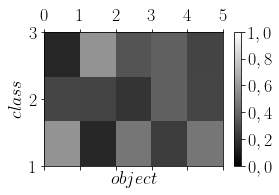
\includegraphics[width=0.3\textwidth]{figures/distr_real.png}}
\subfloat[Модель без учителя]{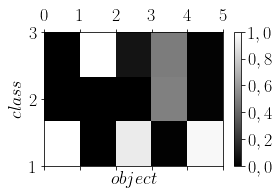
\includegraphics[width=0.3\textwidth]{figures/distr_without_teacher.png}}
\subfloat[Модель с учителем]{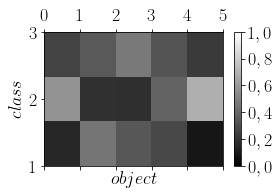
\includegraphics[width=0.3\textwidth]{figures/distr_with_teacher.png}}
\end{figure}


\begin{table}[]
\begin{center}
\resizebox{\textwidth}{!}{
\begin{tabular}{|l|c|c|c|c|c|c|}
\hline
\multicolumn{1}{|c|}{Выборка} & Модель      & \begin{tabular}[c]{@{}c@{}}Кросс-Энтропийная\\ ошибка\end{tabular} & \begin{tabular}[c]{@{}c@{}}{\color{blue}Кросс-Энтропийная} \\ {\color{blue}ошибка с реальными}\\ {\color{blue}вероятностями}\end{tabular} & \begin{tabular}[c]{@{}c@{}}{\color{red}Вероятностная}
\\ {\color{red}разница}\end{tabular} & Точность            & \begin{tabular}[c]{@{}c@{}}Число\\ Параметров\end{tabular} \\ \hline\hline
\multirow{2}{*}{FashionMnist} & с учителем  & $0{,}453\pm0{,}003$                                                & -                                                                                             & $0{,}84\pm0{,}13$                                               & $0{,}842\pm0{,}002$ & 7850                                                       \\ \cline{2-7} 
                              & без учителя & $0{,}461\pm0{,}005$                                                & -                                                                                             & $0{,}86\pm0{,}18$                                               & $0{,}841\pm0{,}002$ & 7850                                                       \\ \hline \hline
\multirow{2}{*}{Systetic}     & с учителем  & $0{,}618\pm0{,}001$                                                & $\mathbf{1{,}17}\pm\mathbf{0{,}05}$                                                                             & $\mathbf{0{,}45}\pm\mathbf{0{,}20}$                                               & $0{,}828\pm0{,}002$ & 33                                                         \\ \cline{2-7} 
                              & без учителя & $0{,}422\pm0{,}002$                                                & $2{,}64\pm0{,}02$                                                                             & $0{,}75\pm0{,}22$                                               & $0{,}831\pm0{,}001$ & 33                                                         \\ \hline \hline
\multirow{2}{*}{Twiter}       & с учителем  & $0{,}489\pm0{,}003$                                               & -                                                                                             & $0{,}79\pm0{,}17$                                               & $0{,}764\pm0{,}005$ & 1538                                                       \\ \cline{2-7} 
                              & без учителя &  $0{,}501\pm0{,}006$                                                & -                                                                                             & $0{,}83\pm0{,}22$                                               & $0{,}747\pm0{,}004$ & 1538                                                       \\ \hline 
\end{tabular}
}
\end{center}
\end{table}

Точность предсказания модели ученика и учителя на одном уровне.\\
{\color{blue}Модель с учителем аппроксимирует истинные вероятности классов.}\\
{\color{red}Модель с учителем имеет меньшую разницу между вероятностями классов, то есть вероятность не концентрируются в одном классе.}
\end{frame}

\begin{comment}
%---------------------------------------------------------------------------------
\begin{frame}{Анализ решения задачи сопоставления структур моделей с разным размером скрытых слоев}
%{Анализ правдоподобия выборки, сопоставления моделей с разным размером скрытых слоев}
\justifying
Вид суперпозиции модели учителя:
$$
f\bigr(\mathbf{x}\bigr) = \bm{\sigma} \circ \mathbf{U}_3\circ \bm{\sigma} \circ \mathbf{U}_2\circ\bm{\sigma}\circ \mathbf{U}_1\mathbf{x},
$$
Вид суперпозиции модели ученика:
$$
g = \bm{\sigma} \circ \mathbf{W}_3 \circ \bm{\sigma} \circ \mathbf{W}_2 \circ \bm{\sigma} \circ \mathbf{W}_1, \quad \mathbf{W}_{1} \in \mathbb{R}^{10 \times 10}, \mathbf{W}_{2} \in \mathbb{R}^{10 \times 10},  \mathbf{W}_{3} \in \mathbb{R}^{1 \times 10}.
$$
\begin{table}[]
\begin{center}
\resizebox{0.9\textwidth}{!}{
\begin{tabular}{|l|c|c|c|c|}\cline{1-5}
                  & teacher           & student        & distil-student & distil-student-all \\ \cline{1-5}
Структура         & $[10,100,50,1]$   & $[10,10,10,1]$  & $[10,10,10,1]$ & $[10,10,10,1]$ \\ \cline{1-5}
Число параметров  & 6050                    & 210                   & 210                  & 210 \\ \cline{1-5}
Разность площадей   &   -                         & 0                       & $\mathbf{16559}$              & $\mathbf{16864}$  \\ \cline{1-5}
\end{tabular}
}
\end{center}
\end{table}

Численный анализ: интегральная разность~$\ln p\bigr(\mathbf{y}|\mathbf{X}, \mathbf{w}\bigr)$ по итерациям.

\begin{figure}[h!]
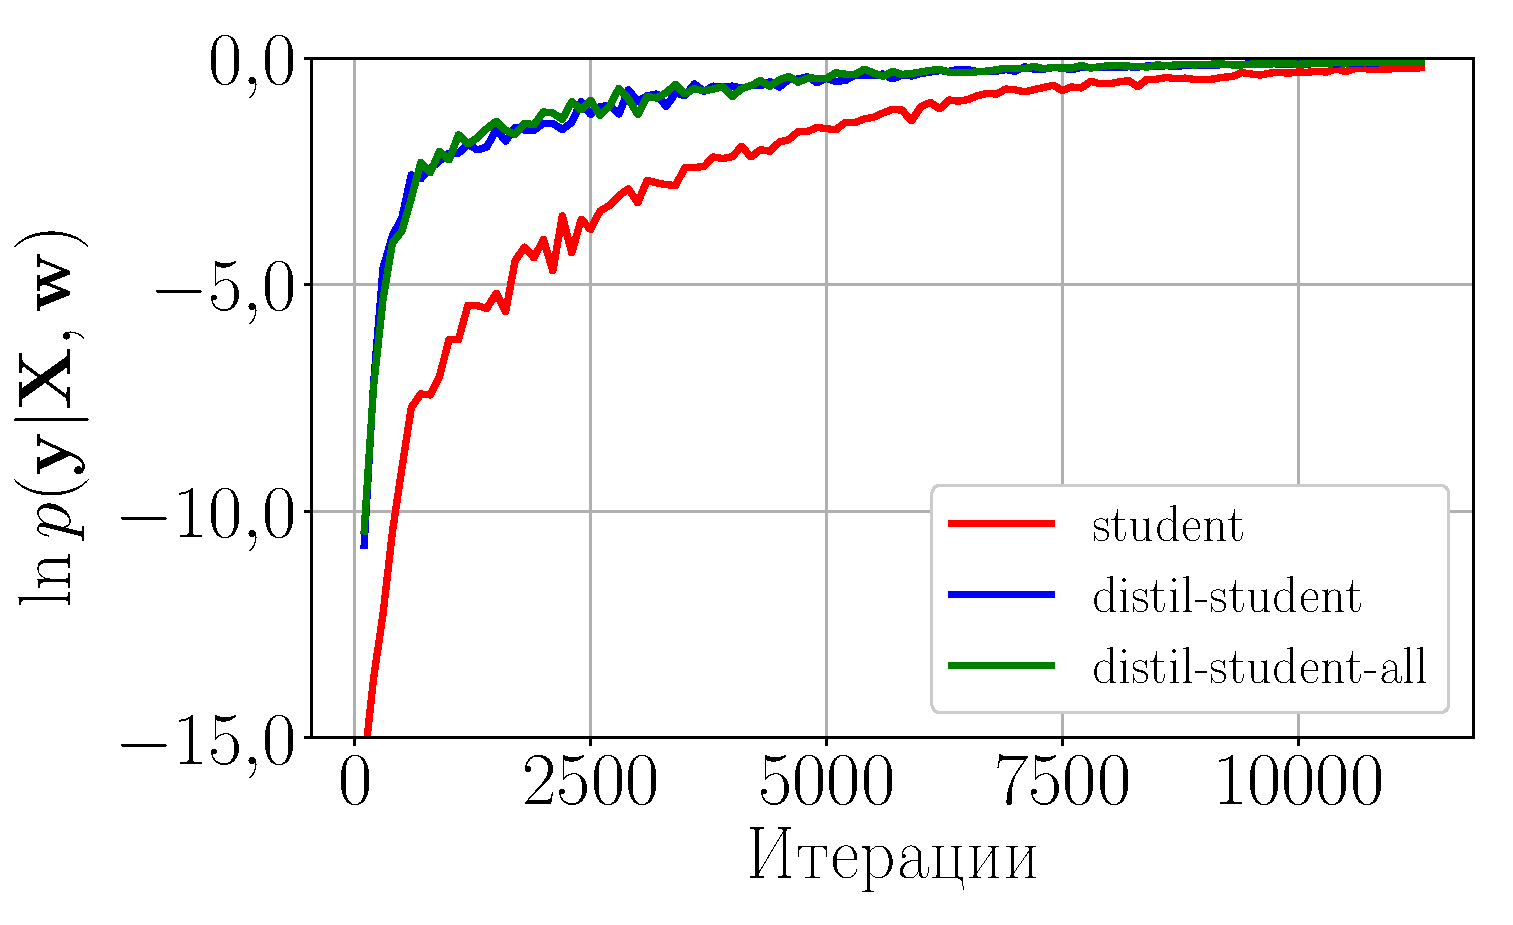
\includegraphics[width=0.4\textwidth]{figures/synthetic_likelihood_3_layers.eps}
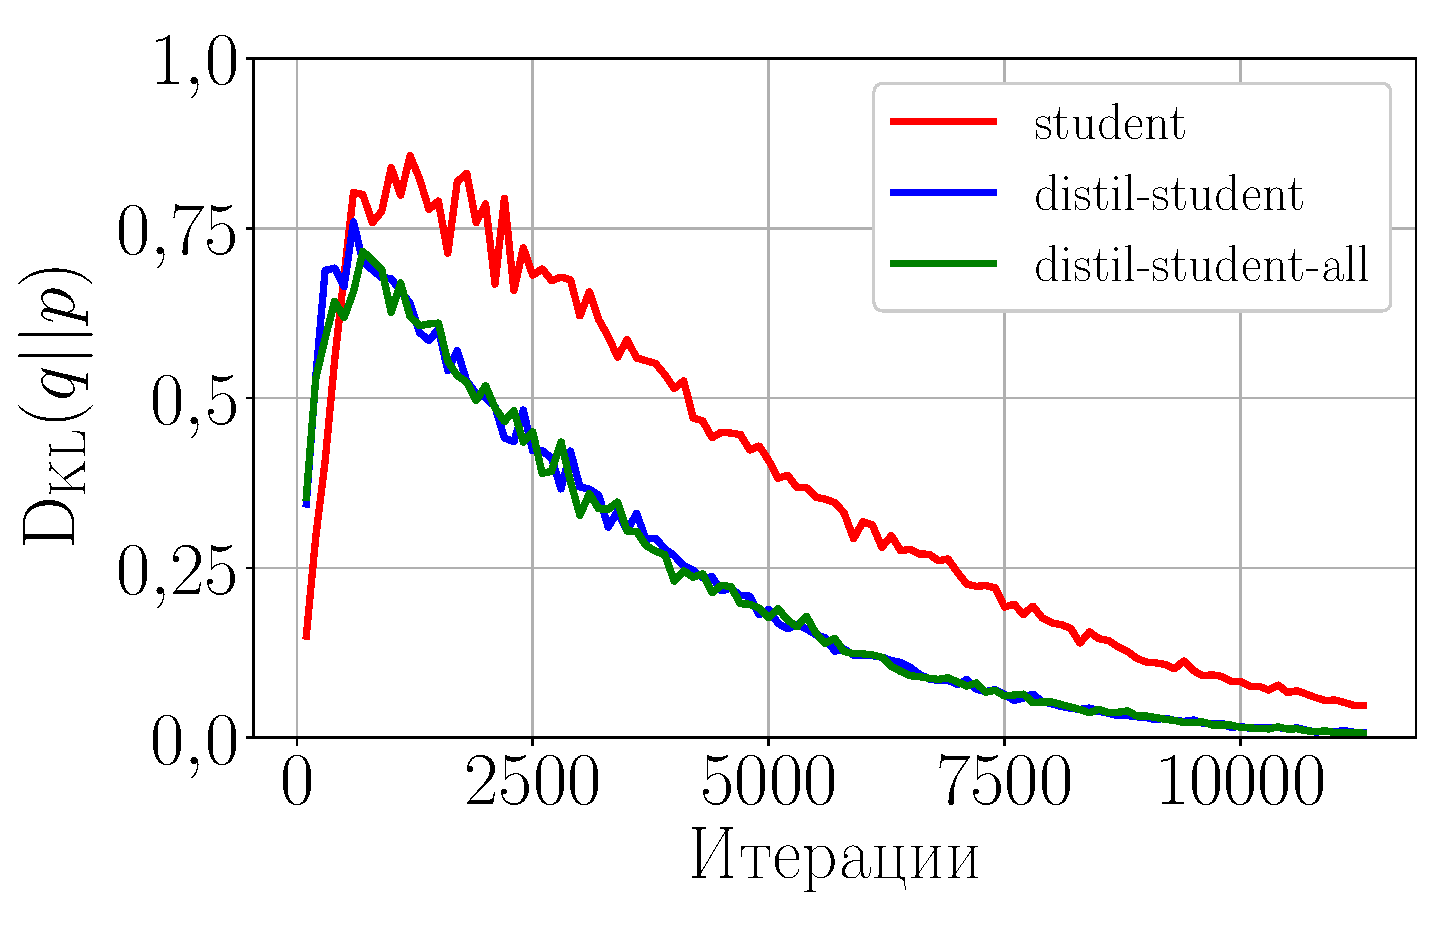
\includegraphics[width=0.4\textwidth]{figures/synthetic_D_KL_3_layers.eps}
\end{figure}

\end{frame}

\end{comment}

%----------------------------------------------------------------------------------------------------------

\begin{frame}{Анализ правдоподобия выборки, сопоставлении моделей с разным числом скрытых слоев}
\justifying
Вид суперпозиции модели учителя:
$$
f\bigr(\mathbf{x}\bigr) = \bm{\sigma} \circ \mathbf{U}_3\circ \bm{\sigma} \circ \mathbf{U}_2\circ\bm{\sigma}\circ \mathbf{U}_1\mathbf{x},
$$
Вид суперпозиции модели ученика:
$$
g = \bm{\sigma} \circ \mathbf{W}_2 \circ \bm{\sigma} \circ \mathbf{W}_1, \quad \mathbf{W}_{1} \in \mathbb{R}^{1 \times 50}, \mathbf{W}_{2} \in \mathbb{R}^{50 \times 10}.
$$
\begin{table}[]
\begin{center}
\resizebox{0.9\textwidth}{!}{
\begin{tabular}{|l|c|c|c|c|}\cline{1-5}
                  & teacher           & student        & distil-student & distil-student-all \\ \cline{1-5}
Структура            & $[10,100,50,1]$   & $[10,50,1]$       & $[10,50,1]$      & $[10,50,1]$ \\ \cline{1-5}
Число параметро    &   6050                       &       550                   &          550               &     550 \\ \cline{1-5}
Разность площадей    &  -                          &  0                      &  $\mathbf{23310}$             & $\mathbf{25506}$ \\ \cline{1-5}
\end{tabular}
}
\end{center}
\end{table}

Численный анализ: интегральная разность~$\ln p\bigr(\mathbf{y}|\mathbf{X}, \mathbf{w}\bigr)$ по итерациям.

\begin{figure}[h!]
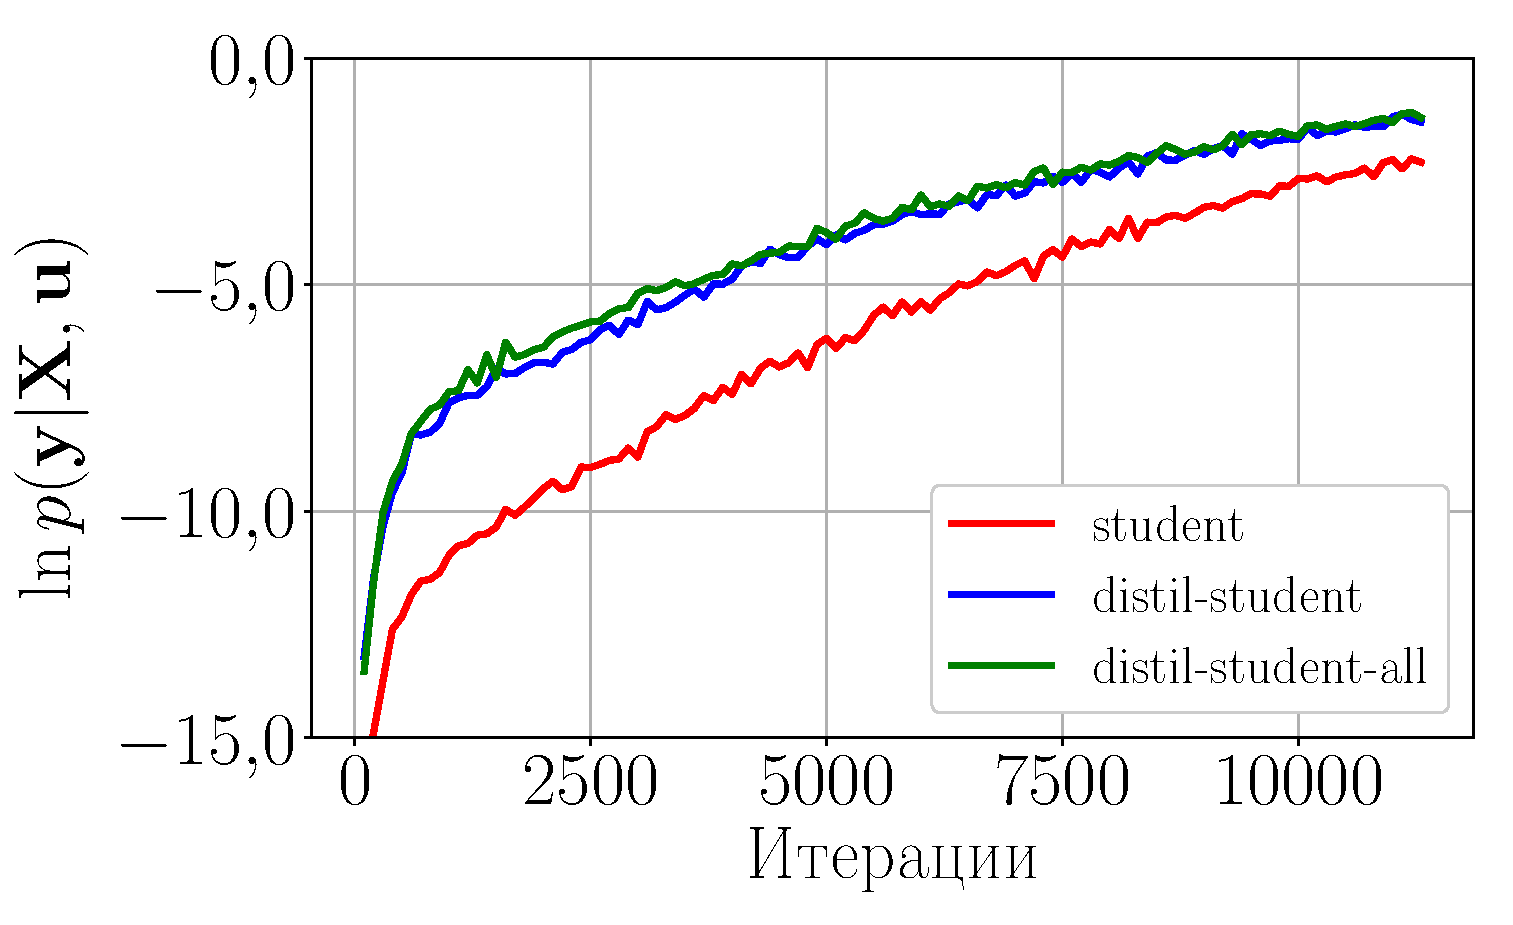
\includegraphics[width=0.4\textwidth]{figures/synthetic_likelihood_2_layers.eps}
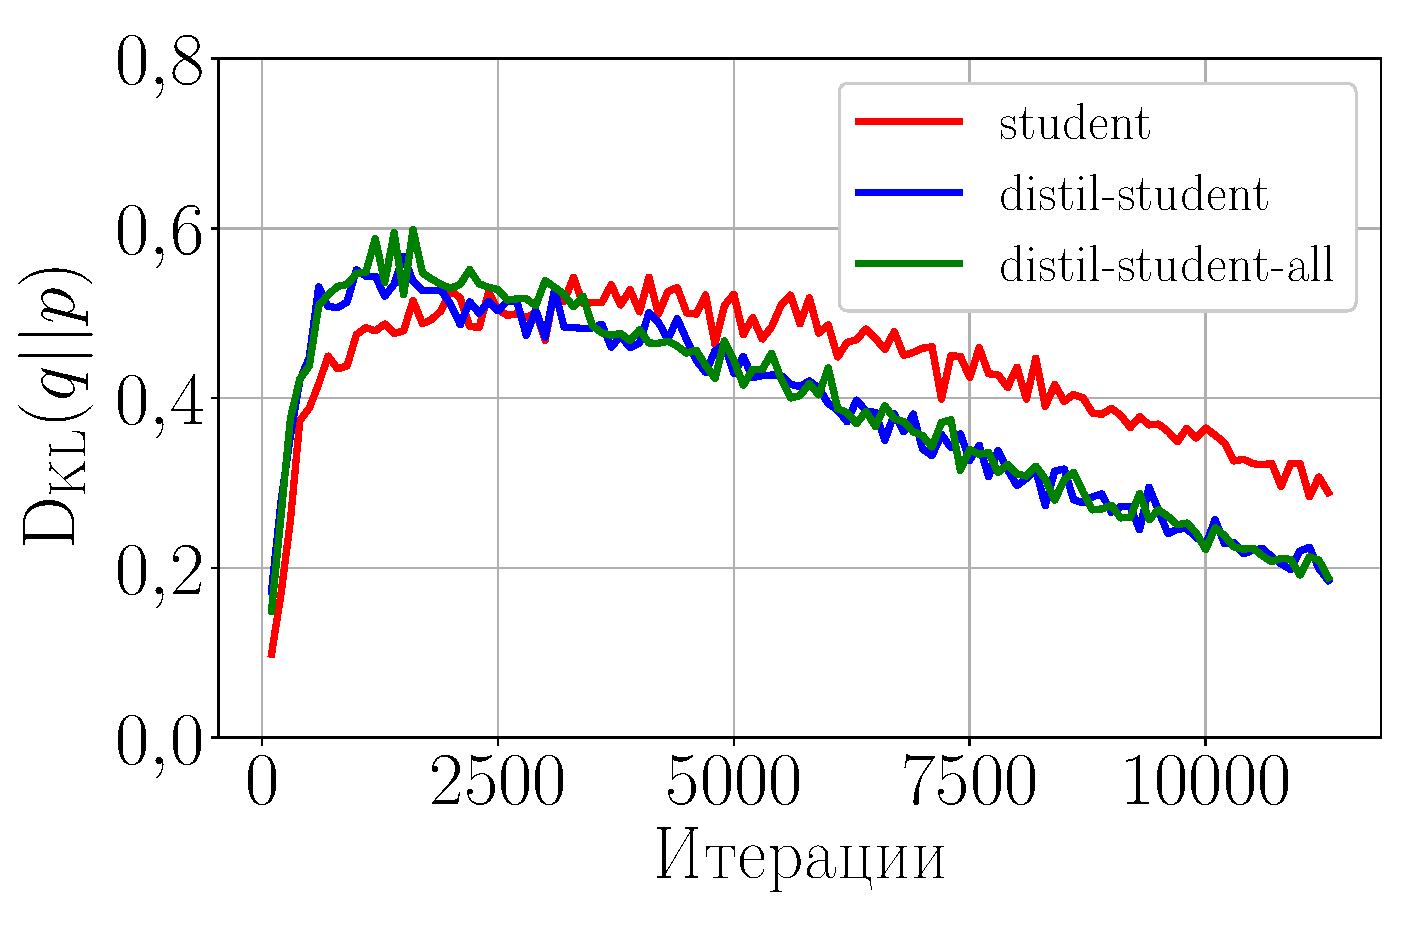
\includegraphics[width=0.4\textwidth]{figures/synthetic_D_KL_2_layers.eps}
\end{figure}

\end{frame}

\begin{comment}

%----------------------------------------------------------------------------------------------------------

\begin{frame}{Анализ сходимости ??чего-к-чему?? дистиллированных моделей}
\justifying

Вид суперпозиции модели учителя:
$
f\bigr(\mathbf{x}\bigr) = \bm{\sigma} \circ \mathbf{U}_3\circ \bm{\sigma} \circ \mathbf{U}_2\circ\bm{\sigma}\circ \mathbf{U}_1\mathbf{x},
$\\
Первый вариант вида суперпозиции модели ученика:
$$
g = \bm{\sigma} \circ \mathbf{W}_3 \circ \bm{\sigma} \circ \mathbf{W}_2 \circ \bm{\sigma} \circ \mathbf{W}_1, \quad \mathbf{W}_{1} \in \mathbb{R}^{10 \times 10}, \mathbf{W}_{2} \in \mathbb{R}^{10 \times 10},  \mathbf{W}_{3} \in \mathbb{R}^{1 \times 10}.
$$
Второй вариант вида суперпозиции модели ученика:
$$
g = \bm{\sigma} \circ \mathbf{W}_2 \circ \bm{\sigma} \circ \mathbf{W}_1, \quad \mathbf{W}_{1} \in \mathbb{R}^{1 \times 50}, \mathbf{W}_{2} \in \mathbb{R}^{50 \times 10}.
$$
Численный анализ: интегральная разность~$\ln p\bigr(\mathbf{y}|\mathbf{X}, \mathbf{w}\bigr)$ по итерациям.

\begin{table}[]
\begin{center}
\resizebox{0.9\textwidth}{!}{
\begin{tabular}{|l|c|c|c|c|}\cline{1-5}
                  & teacher           & student        & distil-student & distil-student-all \\ \cline{1-5}
\multicolumn{5}{|c|}{Эксперимент на синтетической выборке (удаление нейрона)} \\ \cline{1-5}
Структура         & $[10,100,50,1]$   & $[10,10,10,1]$  & $[10,10,10,1]$ & $[10,10,10,1]$ \\ \cline{1-5}
Число параметров  & 6050                    & 210                   & 210                  & 210 \\ \cline{1-5}
Разность площадей   &   -                         & 0                       & $\mathbf{16559}$              & $\mathbf{16864}$  \\ \cline{1-5}
\multicolumn{5}{|c|}{Эксперимент на синтетической выборке (удаление слоя)}  \\ \cline{1-5}
Структура            & $[10,100,50,1]$   & $[10,50,1]$       & $[10,50,1]$      & $[10,50,1]$ \\ \cline{1-5}
Число параметро    &   6050                       &       550                   &          550               &     550 \\ \cline{1-5}
Разность площадей    &  -                          &  0                      &  $\mathbf{23310}$             & $\mathbf{25506}$ \\ \cline{1-5}
\multicolumn{5}{|c|}{Эксперимент на выборке FashionMnist} \\ \cline{1-5}
Структура           & $[784,800,50,10]$& $[784,50,10]$   & $[784,50,10]$  & $[784,50,10]$ \\ \cline{1-5}
Число параметро    &   667700                     &     39700                     &      39700                   &      39700 \\ \cline{1-5}
Разность площадей   & -                           & 0                       &  $\mathbf{1165}$               & $\mathbf{1145} $ \\ \cline{1-5}
\end{tabular}
}
\end{center}
\end{table}
\end{frame}

%----------------------------------------------------------------------------------------------------------
\begin{frame}{Байесовская дистилляция ?? дальше идет сообщение ??}

\begin{figure}[h!]
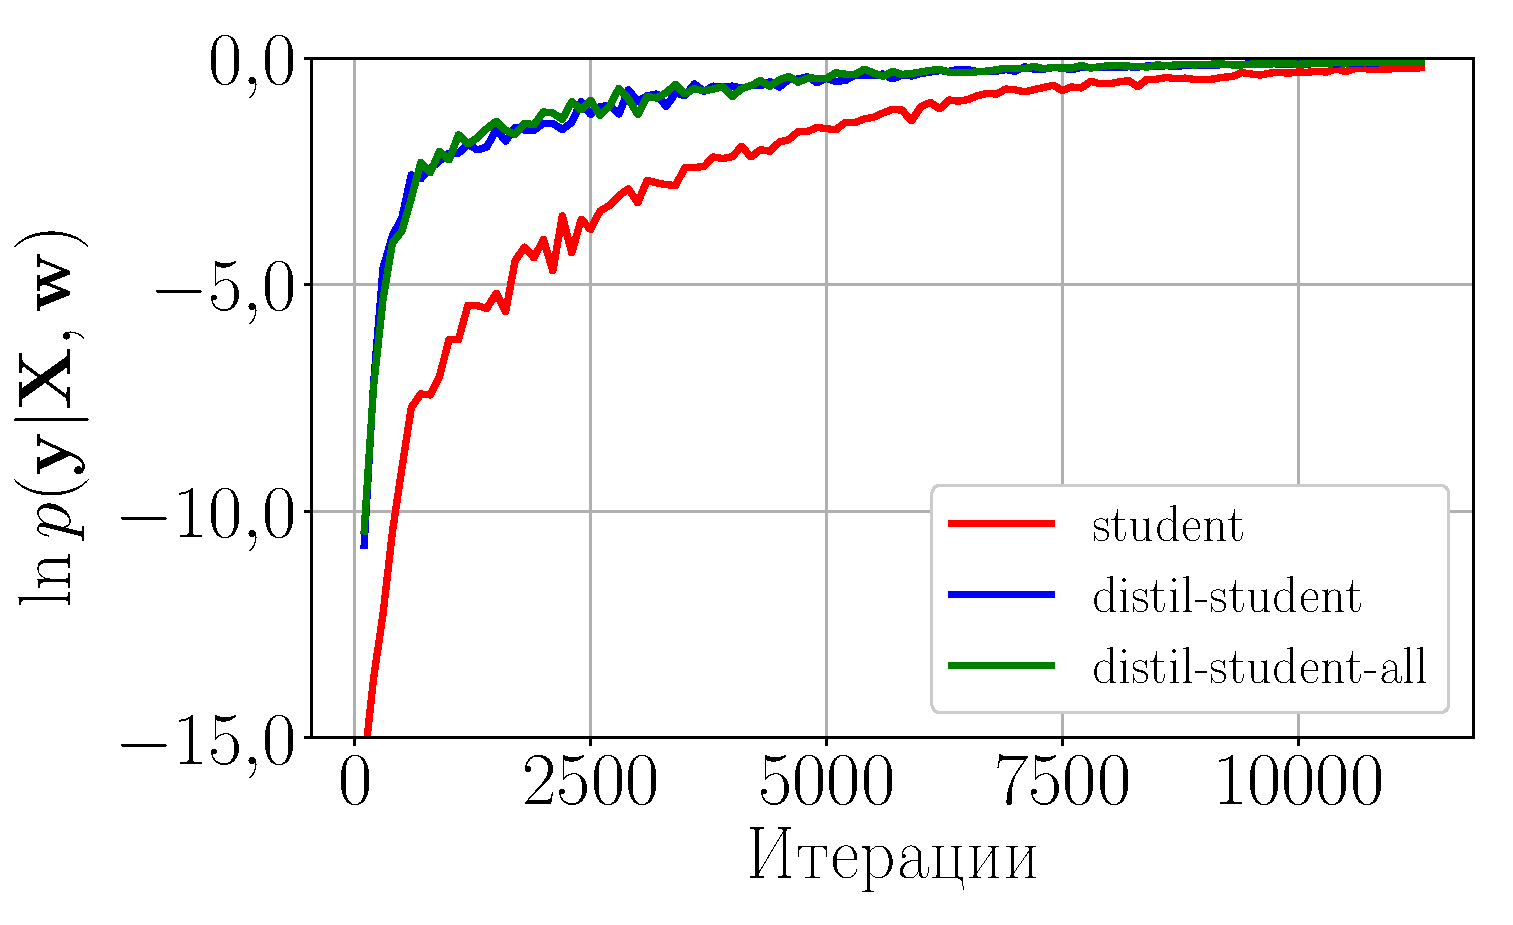
\includegraphics[width=0.4\textwidth]{figures/synthetic_likelihood_3_layers.eps}
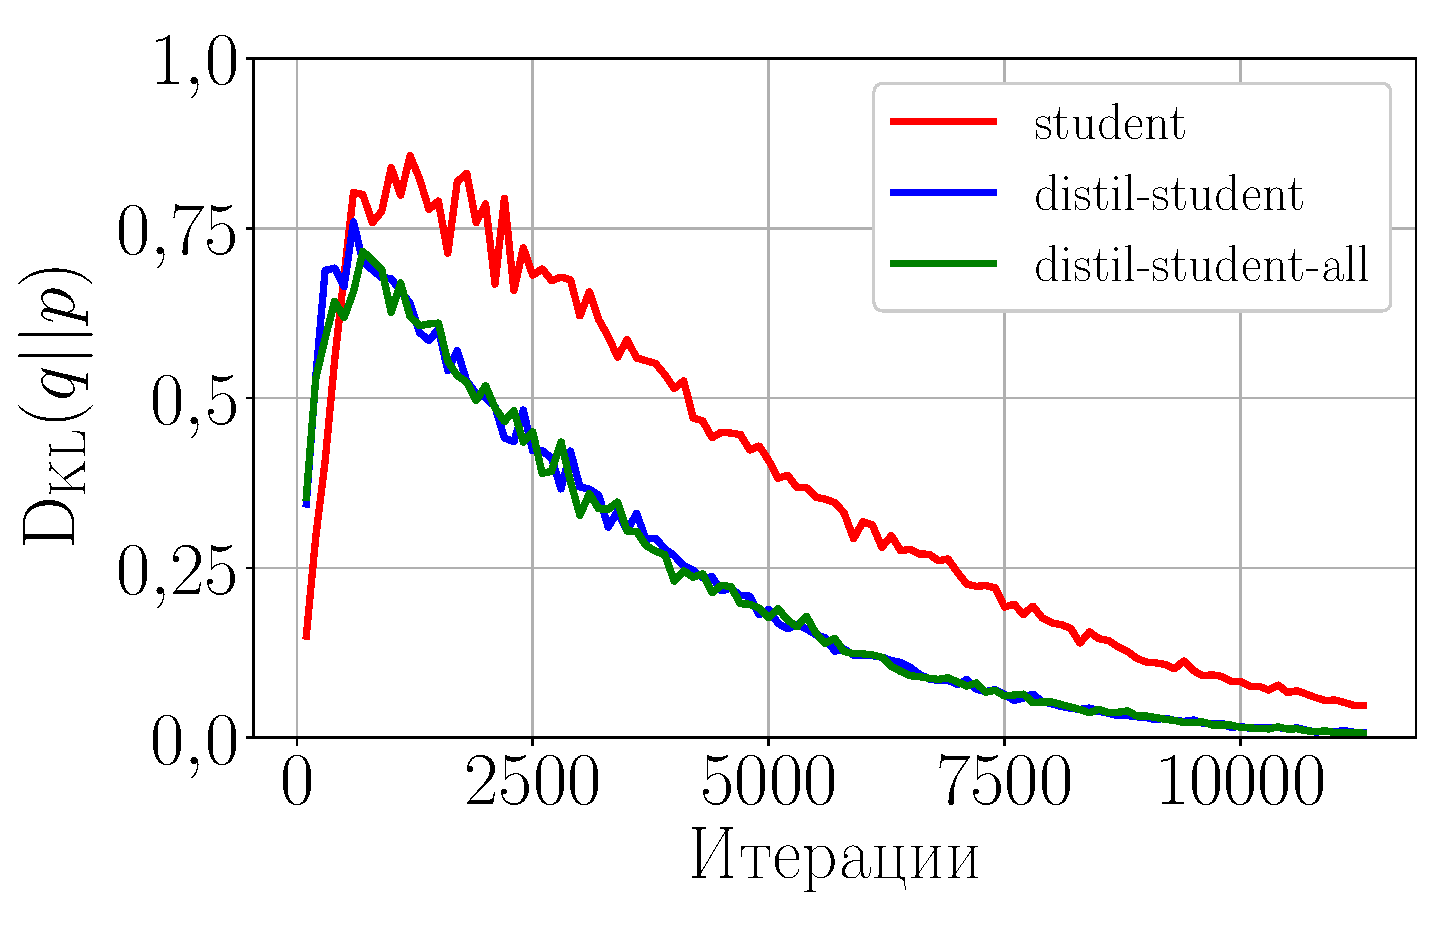
\includegraphics[width=0.4\textwidth]{figures/synthetic_D_KL_3_layers.eps}
\end{figure}
Первый вариант вида суперпозиции модели ученика. Дистиллированная модель имеет большее правдоподобие.

\begin{figure}[h!]
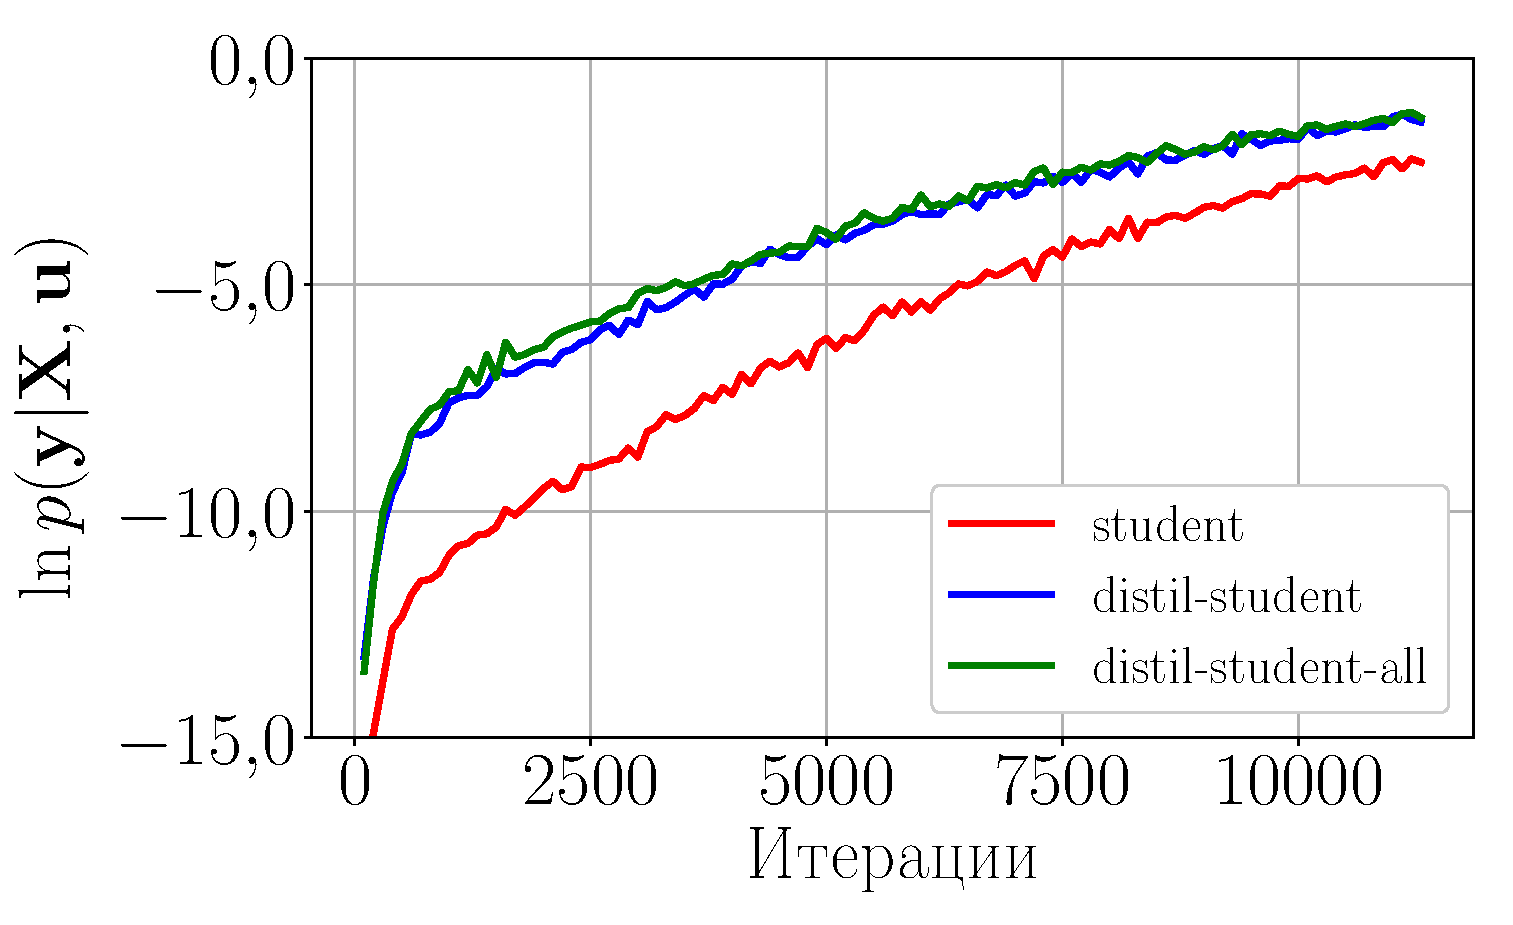
\includegraphics[width=0.4\textwidth]{figures/synthetic_likelihood_2_layers.eps}
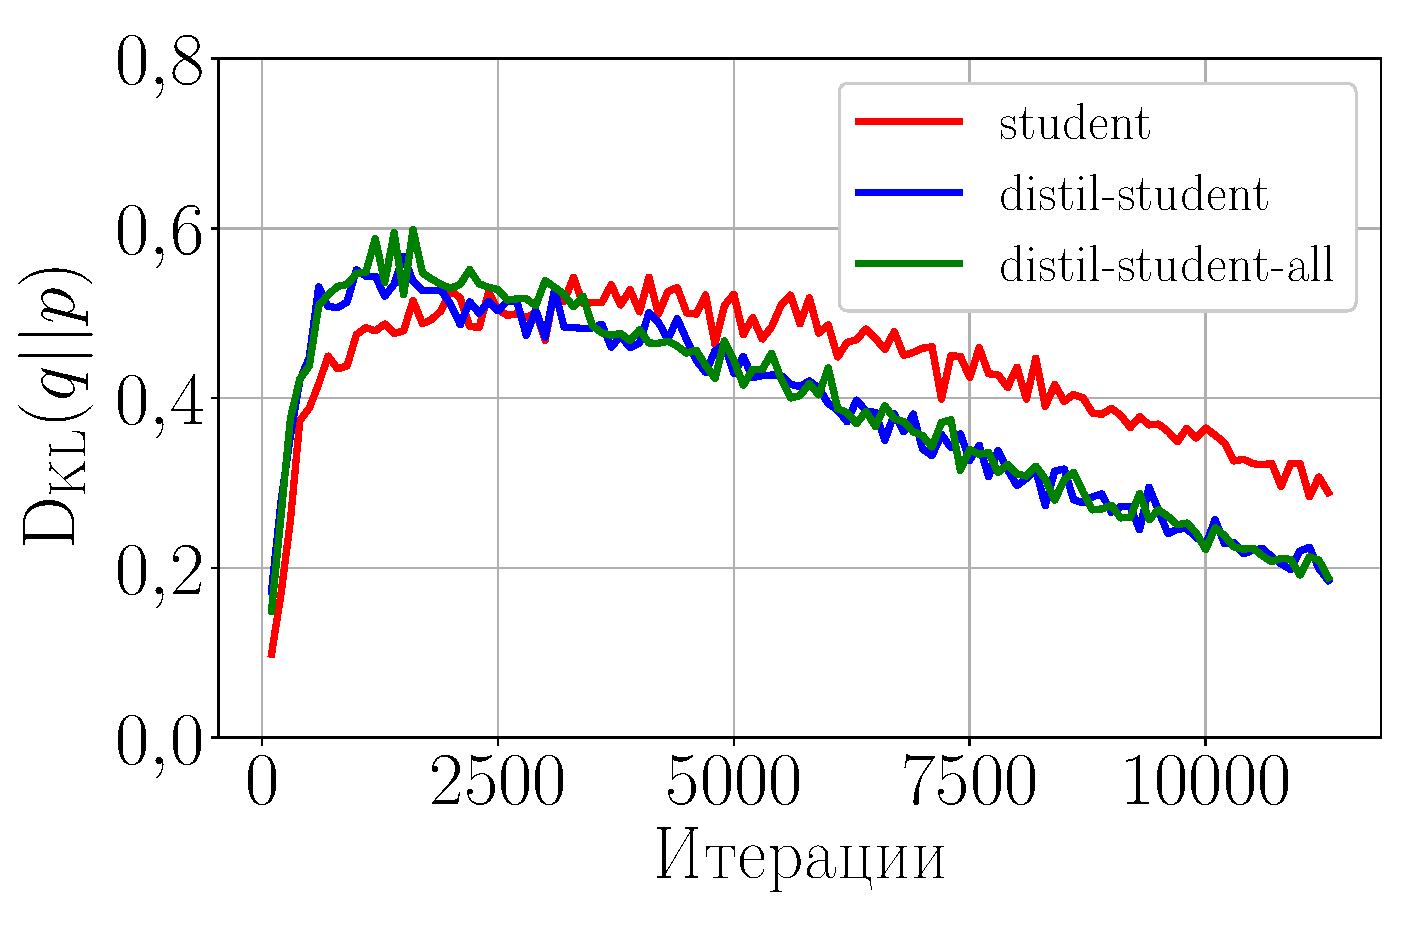
\includegraphics[width=0.4\textwidth]{figures/synthetic_D_KL_2_layers.eps}
\end{figure}
Второй вариант вида суперпозиции модели ученика. Дистиллированная модель имеет большее правдоподобие.

\end{frame}

\end{comment}
%----------------------------------------------------------------------------------------------------------

\begin{frame}{Выносится на защиту}
\justifying
	\begin{enumerate}
	\justifying
	    \item Предложен байесовский метод выбора моделей моделей ученика с использованием моделей учителя с привилегированной и накопленной информации.
        \item Доказаны теоремы о свойствах дистилляции, 
        \begin{itemize}
            \item[---] \emph{теоремы об эквивалентности} для дистилляции моделей в случае задачи регрессии и классификации,
            \item[---] \emph{теоремы о виде априорного распределения} параметров модели ученика в байесовской дистилляции.
        \end{itemize}
        \item Предложен метод сопоставления структур параметрических моделей. Предложен метод выбора априорного распределения параметров модели ученика с использованием апостериорного распределения параметров модели учителя для случаев
        \begin{itemize}
            \item[---] различных размерностей пространств параметров отдельных слоев,
            \item[---] различного в числа слоев нескольких моделей.
        \end{itemize}
        \item Предложены методы задания порядка на множестве параметров моделей
        \begin{itemize}
            \item[---] на основе корреляции параметров,
            \item[---] на основе оценки скорости сходимости параметров.
        \end{itemize}
        \item Предложена вероятностная интерпретации дистилляции моделей глубокого обучения. Исследованы свойства дистилляции моделей глубокого обучения.
	\end{enumerate}
\end{frame}
%----------------------------------------------------------------------------------------------------------

\begin{frame}{Список работ автора по теме диссертации}
\justifying
{
\scriptsize
\textbf{Публикации в журналах ВАК}

\begin{enumerate}
    \item \textit{Грабовой А.В., Стрижов В.В.} Байесовская дистилляция моделей глубокого обучения~// Автоматика и Телемеханика, 2021.
    \item \textit{Грабовой А.В., Стрижов В.В.} Анализ выбора априорного распределения для смеси экспертов~// Журнал Вычислительной математики и математической физики, 2021.
    \item \textit{A. Grabovoy, V. Strijov.} Quasi-periodic time series clustering for human // Lobachevskii Journal of Mathematics, 2020.
    \item \textit{Грабовой А.В., Бахтеев О. Ю., Стрижов В.В.} Введение отношения порядка на множестве параметров аппроксимирующих моделей~// Информатика и ее применения, 2020.
    \item \textit{Грабовой А.В., Бахтеев О.Ю., Стрижов В.В.} Определение релевантности параметров нейросети~// Информатика и ее применения, 2019.
    \item \textit{Грабовой А.В., Стрижов В.В.} Вероятностная интерпретация задачи дистилляции~// Автоматика и Телемеханика (на рецензировании), 2021.
    \item \textit{A. Grabovoy, T. Gadaev, A. Motrenko, V. Strijov} Numerical methods of minimum sufficient sample size estimation for linear models~// Lobachevskii Journal of Mathematics (на рецензировании), 2021.
    \item \textit{Bazarova A.I., Grabovoy A.V., Strijov V.V.} Analysis of the properties of probabilistic models in learning problems with an expert~// Journal of Computational Mathematics (на рецензировании), 2021.
\end{enumerate}

\textbf{Выступления с докладом}
\begin{enumerate}
    \item Задача обучения с экспертом для построения интерпретируемых моделей машинного обучения, Международная конференция <<Интеллектуализация обработки информации>>, 2020.
    \item Привилегированная информация и дистилляция моделей, Всероссийская конференция <<63-я научная конференция МФТИ>>, 2020.
    \item Введение отношения порядка на множестве параметров нейронной сети, Всероссийская конференция <<Математические методы распознавания образов ММРО>>, 2019.
    \item Анализ априорных распределений в задаче смеси экспертов, Всероссийская конференция <<62-я научная конференция МФТИ>>, 2019.
    \item Поиск оптимальной модели при помощи алгоритмов прореживания, Всероссийская конференция <<61-я научная конференция МФТИ>>, 2018.
    \item Автоматическое определение релевантности параметров нейросети, Международная конференция <<Интеллектуализация обработки информации>>, 2018.
\end{enumerate}
}
\end{frame}
%----------------------------------------------------------------------------------------------------------

\end{document} 